\documentclass[notes]{subfiles}

\begin{document}
	\addcontentsline{toc}{section}{1.5 - The Limit of a Function}
	\refstepcounter{section}
	\fancyhead[RO,LE]{\bfseries \large\nameref{cs15}} 
	\fancyhead[LO,RE]{\bfseries \currentname}
	\fancyfoot[C]{{}}
	\fancyfoot[RO,LE]{\large \thepage}	%Footer on Right \thepage is pagenumber
	\fancyfoot[LO,RE]{\large Chapter 1.5}
	
	
\section*{The Limit of a Function}\label{cs15}
	\subsection*{Before Class}
	\addcontentsline{toc}{subsection}{Before Class}
	\subsubsection*{Motivating Example}
	\addcontentsline{toc}{subsubsection}{Motivating Example}
		\begin{ex}
			Consider the function $f(x) = x^3 -2x+1$.  A table of its values (to 6 decimal places) are given below:
				\begin{center}
					{\renewcommand{\arraystretch}{1.2}
					\begin{tabular}{|P{1in}|P{1in}||P{1in}|c|}\hline
						$x$ & $f(x)$ & $x$ & $f(x)$ \\ \hline
						1.0 & 0.000000 & 3.0 & 22.000000 \\ \hline
						1.5 & 1.375000 & 2.5 & 11.625000\\ \hline
						1.8 & 3.232000& 2.2 & 7.248000\\ \hline
						1.9 & 4.059000& 2.1 & 6.061000\\ \hline
						1.95 & 4.514875& 2.05& 5.515125\\ \hline
						1.99 & 4.900599& 2.01& 5.100601\\ \hline
						1.999 & 4.990006& 2.001& 5.010006\\ \hline
					\end{tabular}	
					}
				\end{center}
			Describe what is happening to the output values as $x$ approaches 2.
		\end{ex}
			\vs{1}
			
	\subsubsection*{The Limit}
	\addcontentsline{toc}{subsubsection}{The Limit}
		\begin{defn}[Intuitive Definition of a Limit]
			Suppose $f(x)$ is defined when $x$ is near the input $a$.  We write
				\showto{ins}{
					\[\ds\lim_{x\to a} f(x) = L \qquad f(x)\to L\text{ as }x\to a\]
				}
				\showto{st}{
					\\ \vspace{.5in}
				}
			and say
				\showto{ins}{
					\begin{center}
						``the limit of $f(x)$, as $x$ approaches $a$, equals $L$''\\[2pt]
						``$f(x)$ approaches $L$ as $x$ approaches $a$''\\[10pt]
					\end{center}
				}
				\showto{st}{
					\\ \vspace{1in}
				}
			if we can make the values of $f(x)$ arbitrarily close to $L$ by restricting $x$ to be sufficiently close to $a$ (on either side of $a$) but not equal to $a$ itself.
		\end{defn}
			
		There is a more rigorous definition given in \S1.7.  One important aspect of the definition of a limit is that we do not require the function to \emph{exist} at the input $a$.  
			\vs{.5}
			\newpage
		\begin{rmk}[A Word About Notation]
			In mathematics, notation is the way you succinctly communicate your ideas.  Notation is part of the ``language'' of math$-$proper notation ensures proper communication.  Please pay very careful attention to how I am writing the notation in class.  \\
			Notation can be a confusing aspect of mathematics$-$that's ok.  It happens for Calculus I students and even for tenured professors.  If you have any questions, please refer to your notes and/or ask me!  I am happy to help you navigate things that are confusing or don't make sense to you.
		\end{rmk}
		\begin{ex}
			Draw three graphs so that the limit $L$ is defined at the input $a$, but $f(a)$ is distinct at all three points.  This illustrates three possibilities when dealing with limits.
		\end{ex}
			\vs{2}
			
		\begin{ex}
			Consider $f(x) = \dfrac{x-1}{x^2-1}$.  What is $\ds \lim_{x\to 1} f(x)$?
			\begin{enumerate}[(a)]
				\item Fill out the table below (using a calculator) to six decimal places.  What do you think the limit will be?  Why?\\
					\begin{center}
						\tabulinesep = 1mm
						\begin{tabu}to .9\textwidth{|X[c]|X[3,c] || X[c] | X[3,c]|}\hline
							$x$		&	$f(x)$		& $x$		& $f(x)$\\ \hline
									& 				&			& \\
							0		& 				& 2			& \\
									&				& 			& \\ \hline
									& 				&			& \\
							0.5		& 				& 1.5		& \\
									&				& 			& \\ \hline
									& 				&			& \\
							0.75	& 				& 1.25		& \\
									&				& 			& \\ \hline
									& 				&			& \\
							0.99	& 				& 1.01		& \\
									&				& 			& \\ \hline				
									\multicolumn{4}{|c|}{}\\						
								\multicolumn{4}{|c|}{$\ds \lim_{x\to 1}f(x) \approx$} \\ 
									\multicolumn{4}{|c|}{}\\ \hline				
						\end{tabu}
					\end{center}
						\newpage
						
				\item Simplify the function.  Can you determine the limit from your simplified version?
					\vs{1}
			\end{enumerate}
		\end{ex}
		\newsec
		
	\subsubsection*{Pre-Class Activities}		
	\addcontentsline{toc}{subsubsection}{Pre-Class Activities}
		\begin{ex}
			What if instead we tweaked the function in the previous example to be 
						\[g(x) = \begin{cases}\dfrac{x-1}{x^2-1} & x\neq 1\\[5pt] 2 & x = 1 \end{cases}\]
					 What will happen to the limit?  Explain your answer.
						\vs{1}
		\end{ex}
		
		\begin{ex}
			\begin{enumerate}[(a)]
				\item Translate the expression $\ds \lim_{x\to 3} f(x) = 7$ from math into English.  Explain the sentence you wrote. 
					\vs{1}
				\item Is it possible for $f(3)$ to be $-10$ instead of 7?  Why or why not?
					\vs{1}
			\end{enumerate}
		\end{ex}
			\newpage

	\subsection*{In-Class}
	\addcontentsline{toc}{subsection}{In-Class}
	\subsubsection*{One-Sided Limits}
	\addcontentsline{toc}{subsubsection}{One-Sided Limits}
		When we developed the intuition of a limit, we looked at input values which were smaller and larger than our desired input.  These values are to the \emph{left} and \emph{right} of our input; secretly, we were taking \emph{one-sided limits}.
		\begin{defn}[One-Sided Limits]
			Suppose $f(x)$ is defined when $x$ is near the input $a$.  We write
				\showto{ins}{
					\[\lim_{x\to a^+} f(x) = L\]			
				}
				\showto{st}{
					\\ \vspace{.6in}
				}
			and say
				\showto{ins}{
					\begin{center}
						``the limit of $f(x)$, as $x$ approaches $a$ from the right, equals $L$''\\[2pt]
						``$f(x)$ approaches $L$ as $x$ approaches $a$ from the right''\\[10pt]
					\end{center}
				}
				\showto{st}{
					\\ \vspace{1in}
				}
			if we can make the values of $f(x)$ arbitrarily close to $L$ by restricting $x$ to be sufficiently close to $a$ (using $x < a$).  We write
				\showto{ins}{
					\[\lim_{x\to a^-} f(x) = L\]			
				}
				\showto{st}{
					\\ \vspace{.6in}
				}
			and say
				\showto{ins}{
					\begin{center}
						``the limit of $f(x)$, as $x$ approaches $a$ from the left, equals $L$''\\[2pt]
						``$f(x)$ approaches $L$ as $x$ approaches $a$ from the left''\\[10pt]
					\end{center}
				}
				\showto{st}{
					\\ \vspace{.75in}
				}
			if we can make the values of $f(x)$ arbitrarily close to $L$ by restricting $x$ to be sufficiently close to $a$ (using $x > a$).
		\end{defn}
		\begin{rmk}[Existence of a Limit]
			A function $f(x)$ has a limit at $x = c$ if and only if
			\showto{ins}{
				\fbox{its one-sided limits exist and agree.}
			}
			\showto{st}{
				\\[20pt] \vspace*{2in}
			}
		\end{rmk}
			\vs{1}
			\newpage
	
		\begin{ex} \label{discontinuity} Use the graph of $g$ to answer the following: 
			\begin{center}
			\begin{minipage}{.45\textwidth}
				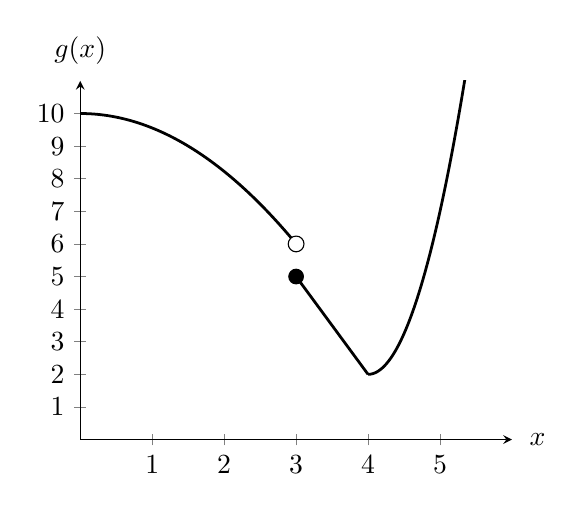
\begin{tikzpicture}
				\begin{axis}[
					scale = .8,
					axis x line = middle,
					axis y line = middle,
	    			every axis y label/.style={at={(ticklabel cs:1.15)}},
	    			ytick = {1,2,...,10},
					y label style={at={(axis description cs:0,1.15)},anchor=north},
	    			ylabel = {$g(x)$},
	    			ymin = 0, ymax = 11,
    				every axis x label/.style= {at ={(ticklabel cs:1)}},
    				xtick = {1,2,3,4,5},
    				x label style={at={(axis description cs:1.1,0)},anchor=east},
    				xlabel = {$x$},
    				xmin = 0, xmax = 6			
				]
					\addplot [line width=1pt,smooth,samples=100,domain=0.:2.93] {(-.444)*x^2 + 10}; % plots first piece of function
					\coordinate (circle1) at (3,6);
					\addplot[line width = 1pt, smooth, samples = 100, domain = 3.0:4.0] {-3.*x + 14.}; %plot second piece
					\coordinate (circle2) at (3,5);
					\addplot[->,line width = 1pt, smooth, samples = 100, domain = 4.0:6.0] {5*(x - 4)^2 + 2}; %plot third piece
				\end{axis}
				\fill[white] (circle1) circle (.1);
				\draw (circle1) circle (.1);
				\fill (circle2) circle (.1);
			\end{tikzpicture}
			\end{minipage}\hspace{20pt}
			\begin{minipage}{.45\textwidth}
				\begin{multicols*}{2}
					\begin{enumerate}[(a)]
						\setlength\itemsep{.75in}
						\item $\ds \lim_{x\to 4^-} g(x)=$     
						\item $\ds \lim_{x\to 4^+} g(x)=$     
						\item $\ds \lim_{x\to 4} g(x)=$ 
							\columnbreak  
						\item $\ds \lim_{x\to 3^-} g(x)=$     
						\item $\ds \lim_{x\to 3^+} g(x)=$     
						\item $\ds \lim_{x\to 3} g(x)=$   
							\raggedcolumns
					\end{enumerate}
				\end{multicols*}
			\end{minipage}
			\end{center}
		\end{ex}
			\vs{1}
			
		\begin{ex}
			Use a calculator to examine the limit behavior of the function $r(p) = \dfrac{p^2-64}{p+8}$ at $p = -8$.  Record your answers will full decimal accuracy, and round your final answer to the thousandths place, if necessary.\\
			\begin{center}
				\begin{minipage}{.45\textwidth}
					\tabulinesep=1mm
					\begin{tabu}{|X[c]|X[1.5,c]|}\hline
						$p$ 						& $r(p)$ \\ \hline
												& \\
						$-8.1$					& \\ 
												& \\ \hline
												& \\
						$-8.01$	& \\
												& \\ \hline 
												& \\
						$-8.001$	& \\ 
												& \\ \hline
												& \\ 
						$-8.0001$	& \\ 
												& \\ \hline
												& \\
						$-8.00001$	&\\
												&\\ \hline\hline
												&\\
						$\ds \lim_{p\to -8^-}r(p)  =$ & \\
												&\\ \hline
					\end{tabu}
				\end{minipage}
				\begin{minipage}{.45\textwidth}
					\tabulinesep=1mm
					\begin{tabu}{|X[c]|X[1.5,c]|}\hline
						$p$ 		& $r(p)$ \\ \hline
								& \\
						$-7.9$		& \\ 
								& \\ \hline
								& \\
						$-7.99$	& \\
								& \\ \hline 
								& \\
						$-7.999$	& \\ 
								& \\ \hline
								& \\ 
						$-7.9999$	& \\ 
								& \\ \hline
								& \\
						$-7.99999$	&\\
								&\\ \hline\hline
								&\\
						$\ds \lim_{p\to -8^+}r(p) =$ & \\
								&\\ \hline
					\end{tabu}
				\end{minipage}
					\vs{1}
				\[\lim_{p\to -8}r(p)= \blank{3}\]
					\vs{.25}
			\end{center}					
		\end{ex}
			\newpage
			
	\subsubsection*{Infinite Limits}
	\addcontentsline{toc}{subsubsection}{Infinite Limits}
		\begin{ex}
			Estimate $\displaystyle \lim_{x\to 0} -\dfrac{1}{x^2}$.
			\begin{center}
				\begin{minipage}{.45\textwidth}
					\tabulinesep=1mm
					\begin{tabu}{|X[c]|X[1.5,c]|}\hline
						$x$ 						& $-\dfrac{1}{x^2}$ \\ \hline
												& \\
						$-0.1$					& \\ 
												& \\ \hline
												& \\
						$-0.01$	& \\
												& \\ \hline 
												& \\
						$-0.001$	& \\ 
												& \\ \hline
												& \\ 
						$-0.0001$	& \\ 
												& \\ \hline
												& \\
						$-0.00001$	&\\
												&\\ \hline\hline
												&\\
						$\ds \lim_{x\to 0^-}\lrpar{-\dfrac{1}{x^2}} =$ & \\
												&\\ \hline
					\end{tabu}
				\end{minipage}
				\begin{minipage}{.45\textwidth}
					\tabulinesep=1mm
					\begin{tabu}{|X[c]|X[1.5,c]|}\hline
						$x$ 						& $-\dfrac{1}{x^2}$ \\ \hline
												& \\
						$ 0.1$					& \\ 
												& \\ \hline
												& \\
						$ 0.01$	& \\
												& \\ \hline 
												& \\
						$ 0.001$	& \\ 
												& \\ \hline
												& \\ 
						$ 0.0001$	& \\ 
												& \\ \hline
												& \\
						$ 0.00001$	&\\
												&\\ \hline\hline
												&\\
						$\ds \lim_{x\to 0^+}\lrpar{-\dfrac{1}{x^2}} =$ & \\
												&\\ \hline
					\end{tabu}
				\end{minipage}
					\vs{.25}
				\[\lim_{x\to 0}\lrpar{-\dfrac{1}{x^2}}= \blank{3}\]
					\vs{.25}
			\end{center}	
		\end{ex}		
			\vs{.25}
			
		\begin{question}
			What is different about these outputs than in our previous examples?
		\end{question}
			\vs{1}
			
		\begin{rmk}[Notation]
			\showto{ins}{
				We use the notation $\infty$ or $-\infty$ to indicate a value which gets arbitrarily large.  IT IS NOT A NUMBER!
			}
			\showto{st}{
				\\ \vspace{1in}
			}
		\end{rmk}
			\newpage
			
		\begin{defn}[Intuitive Definition of an Infinite Limit]
			Let $f$ be a function defined on both sides of $a$, except possibly at $a$ itself.  If the values of $f(x)$ can be made arbitrarily large, by taking $x$ sufficiently close to $a$ (but not equal to $a$).  We denote this as
				\showto{ins}{
					\[\lim_{x\to a} f(x) = \infty\]
				}
				\showto{st}{
					\\ \vspace{1in}
				}
			If the values can be made arbitrarily negative, we denote this as \newline
				\showto{ins}{
					\[\lim_{x\to a} f(x) = -\infty\]
				}
				\showto{st}{
					\\ \vspace{1in}
				}
			One-sided limits are defined similarly.
		\end{defn}
					
		\begin{ex}
			Sketch an example of each of the following:
			\begin{center}
				\begin{enumerate}[(a)]
				\setlength\itemsep{1.2in}
					\begin{multicols*}{2}
						\item $\displaystyle \lim_{x\to a^-} f(x) = \infty$
							 
						\item $\displaystyle \lim_{x\to a^+} f(x) = \infty$
							 
						\item $\displaystyle \lim_{x\to a} f(x) = \infty$
							\columnbreak
							
						\item $\displaystyle \lim_{x\to a^-} f(x) = -\infty$
							 
						\item $\displaystyle \lim_{x\to a^+} f(x) = -\infty$
							 
						\item $\displaystyle \lim_{x\to a} f(x) = -\infty$
							\raggedcolumns
												 
					\end{multicols*}
				\end{enumerate}
			\end{center}
		\end{ex}

			\newpage
			
		\begin{defn}[Vertical Asymptote]
			The vertical line $x = a$ is called a \textbf{vertical asymptote} of the curve $y = f(x)$ if at least one of the following statements is true:
			\showto{ins}{
				\[\lim_{x\to a} f(x) = \infty \qquad \lim_{x\to a^-} f(x) = \infty \qquad \lim_{x\to a^+}f(x) = \infty\]
				\[\lim_{x\to a} f(x) = -\infty \qquad \lim_{x\to a^-} f(x) = -\infty \qquad \lim_{x\to a^+} f(x) = -\infty\]
			}
			\showto{st}{
				\\ $ $\vspace*{1.5in}
			}
		\end{defn}
		
		\begin{ex}
			Find the left- and right-hand limits for the function $f(x) = \dfrac{4x}{x-6}$ at $x = 6$.  
				\vs{1}
		\end{ex}
			
		\begin{ex}
			In the theory of relativity, the mass of a particle with velocity $v$ is given by $m = \dfrac{m_0}{\sqrt{1-v^2/c^2}}$, where $m_0$ is the mass of the particle at rest and $c$ is the speed of light.  What happens as $v\to c^-$?
				\vs{1}
		\end{ex}
			\newpage
			
	\subsection*{After Class}
	\addcontentsline{toc}{subsection}{After Class}
		\begin{ex}
			For the function $g$ whose graph is given below, state the value of each quantity (if it exist).  If it does not exist, explain why.\\
			\begin{minipage}{.4\textwidth}
				\includegraphics{1.5fig1}
			\end{minipage}
			\begin{minipage}{.45\textwidth}
				\begin{multicols*}{2}
					\begin{enumerate}[(a)]
						\setlength\itemsep{.75in}
							\item $\ds \lim_{t\to 0^-} g(t)$ 
							\item $\ds \lim_{t\to 0^+} g(t)$
							\item $\ds \lim_{t\to 0} g(t)$
							\item $\ds \lim_{t\to 2^-} g(t)$
								\columnbreak
							\item $\ds \lim_{t\to 2^+} g(t)$
							\item $\ds \lim_{t\to 2} g(t)$
							\item $g(2)$
							\item $\ds \lim_{t\to 4} g(t)$
							\raggedcolumns
					\end{enumerate}
				\end{multicols*}
			\end{minipage}
		\end{ex}
			\vs{1}
		\begin{ex}
			Sketch a graph of an example of a function $f$ that satisfies the given conditions: $\ds \lim_{x\to 0} f(x) = 1$, $\ds \lim_{x\to 3^-} f(x) = -2$, $\ds \lim_{x\to 3^+} f(x) = 2$, $f(0) = -1$, $f(3) = 1$.
		\end{ex}
			\vs{2}
			\newpage 
			
		\begin{ex}
			Determine the limits for the following functions:
			\begin{enumerate}[(a)]
				\item $\ds \lim_{x\to 5^+} \dfrac{x+1}{x-5}$
					\vs{1}
					
				\item $\ds \lim_{x\to 5^-} \dfrac{x+1}{x-5}$
					\vs{1}
					
				\item $\ds \lim_{x\to 2\pi^+} x\csc x$
					\vs{1}
					
			\end{enumerate}
		\end{ex}
	\clearpage
	
\end{document}